\section{Unternehmerischer Kontext}
\subsection{Die adesso orange AG}
\subsubsection{Vorstellung des Unternehmens}
Die adesso orange AG ist ein IT-Beratungsunternehmen, das sich vor allem auf die SAP-Beratung spezialisiert hat. Sie ist ein Tochterunternehmen der Dortmunder adesso SE, das im Jahr 2021 aus einer Fusion der adesso SE mit der in Hameln ansässigen Quanto AG hervorging. Die adesso SE ist eines der größten IT-Dienstleistungs- und Beratungsunternehmen Deutschlands und hat ca. 5600 Mitarbeiter an 44 Standorten in ganz Deutschland und Europa. \footcite[Vgl.][]{adesso-main} \\Die adesso SE wurde im Jahr 1997 als \glqq{}adesso Beratungsgesellschaft für Software-Prozeß-Management mbH\grqq{} gegründet und hatte Ende der 1990er Jahre erste größere Projekte im Versicherungssektor. Im Jahr 2000 wurde die Gesellschaft mit beschränkter Haftung schließlich zu einer Aktiengesellschaft umgewandelt, zu diesem Zeitpunkt hatte sie bereits 100 Mitarbeiter. Ende der 2000er-Jahre hatte die adesso bereits über 500 Mitarbeiter und erschloss zunehmend die internationalen Märkte in ganz Europa. Im Jahr 2012 erwirtschaftete die adesso AG mit ca. 1000 Mitarbeitern über 100 Mio. Euro Umsatz und vergrößerte sich in den nachfolgenden Jahren durch das Gründen von Tochtergesellschaften stetig. Im Jahr 2019 wurde die adesso AG in eine europäische Aktiengesellschaft \glqq{}Societas Europaea\grqq{} (SE) umgewandelt und war, mit über 4000 Mitarbeitern, laut \glqq{}Lünendonk-Liste 2020\grqq{} das größte mittelständische IT-Beratungsunternehmen in Deutschland.\footcite[Vgl.][]{adesso-historie} Im Geschäftsjahr 2020 erreichte die adesso SE eine Umsatzsteigerung von 16 Prozent, im Vergleich zum Vorjahr, auf 523,375 Mio. Euro, wovon ca. 413 Mio. Euro in Deutschland und 110 Mio. Euro im Ausland erwirtschaftet wurden. Von den 523 Mio. Euro waren 60,406 Mio. Euro als Gewinn (EBITDA) zu verzeichnen, was eine Steigerung von 26 Prozent gegenüber dem Vorjahr entspricht. Nach dem Abzug der Abgaben verblieb für das Jahr 2020 ein Konzernergebnis von ca. 21 Mio. Euro.\footcite[Vgl.][S. 4]{adesso2020-report} Besonders sind dabei die Auswirkung der von Anfang 2020 bis dato anhaltenden Covid-19-Pandemie hervorzuheben, die zeitweise zu unterjährigen Wachstumseinbrüchen von bis zu 9,8 Prozent führten. Dies resultierte aus der neu aufgetretenen, allgemeinen Unsicherheit, die unter anderem dazu führte, dass adesso-Kunden Projekte stoppten oder verschoben. Das führte dazu, dass Gesellschaften der adesso SE, wie auch viele andere Unternehmen, im Zeitraum von April bis Juli 2020, teilweise Kurzarbeit anmelden mussten und Maßnahmen zur Liquiditätssicherung, wie zum Beispiel der Vereinbarung von Steuerstundungen, veranlassten. Da es sich bei vielen Kunden von adesso um Versicherungen oder Banken handelt, die dem öffentlichen Sektor entstammen, waren die Auswirkungen der Pandemie nicht allzu prekär, was zu einer Erholung im zweiten Halbjahr führte.\footcite[Vgl.][S. 30f]{adesso2020-report} Im zweiten Halbjahr 2020 wurde auch der Mehrheitserwerb an der Quanto AG in Höhe von 71,4 Prozent durchgeführt, der zu der Fusion und später, im Jahr 2021, zu der Neugründung der adesso orange AG führte.\footcite[Vgl.][S. 15]{adesso2020-report} 
\\Mit der adesso orange AG hat die adesso SE den auf SAP spezialisierten Teil ihres Unternehmens, zusammen mit der ehemaligen Quanto AG, in einem separaten Unternehmen gebündelt, das sich vor allem auf die SAP-Beratung von Banken, Energieversorgern und Versicherungen spezialisiert hat.\footcite[Vgl.][]{ao-main} Derzeit beschäftigt die adesso orange AG ca. 300 Mitarbeiter an den Standorten der adesso SE. Der Hauptsitz befindet sich weiterhin, wie bereits bei der Quanto AG, in Hameln.\footcite[Vgl.][]{ao-karriere}
Die bis 2021 bestehende Quanto AG ging im Jahr 2016 aus dem Zusammenschluss der Firmen \glqq{}Aequitas\grqq{} und \glqq{}Quanto\grqq{} hervor, um gemeinsam größere Kunden zu gewinnen.\footcite[Vgl.][]{ww-quanto} Die Quanto AG hielt bereits Standorte in Hamburg, Kiel, Flensburg, Stuttgart, Heidelberg, Berlin sowie im ungarischen Budapest und Györ und hatte bereits im Jahr 2016 ca. 140 Mitarbeiter. Neben den Bereichen der SAP konzentrierte sich die Quanto AG auch auf das \glqq{}Internet der Dinge\grqq{} und Blockchain-Technologien.\footcite[Vgl.][]{ww-quanto}

\subsubsection{Geschäftsmodell}
Die adesso orange AG ist ein Dienstleistungsunternehmen, das sich auf die SAP-Beratung im öffentlichen Sektor spezialisiert hat. Als Beratungsunternehmen verfolgt die adesso orange AG das Ziel, die Unternehmensstrategie ihrer Kunden in eine angepasste SAP-Architektur zu übersetzen. Die soll geschehen, indem die Unternehmensprozesse in ihrer Gänze betrachtet und analysiert werden und diese anschließend, mit dem mitgebrachten Fachwissen, in eine SAP-Lösung überführt werden.\footcite[Vgl.][]{ao-main} Als Beratungsunternehmen versucht die adesso orange AG als externe Organisation ihren Klienten, durch eine personalisierte Aufarbeitung einer betriebswirtschaftlichen Problemstellung, zu einer Lösung dieses Problems zu verhelfen. Diese Unterstützung kann entweder technischer oder organisatorischer Natur sein und wird an die Erwartung des Klienten angepasst, sowie an das durch die Berater angebotene Leistungsspektrum.\footcite[Vgl.][]{gabler-beratung}
\begin{figure}[h!]
    \centering
    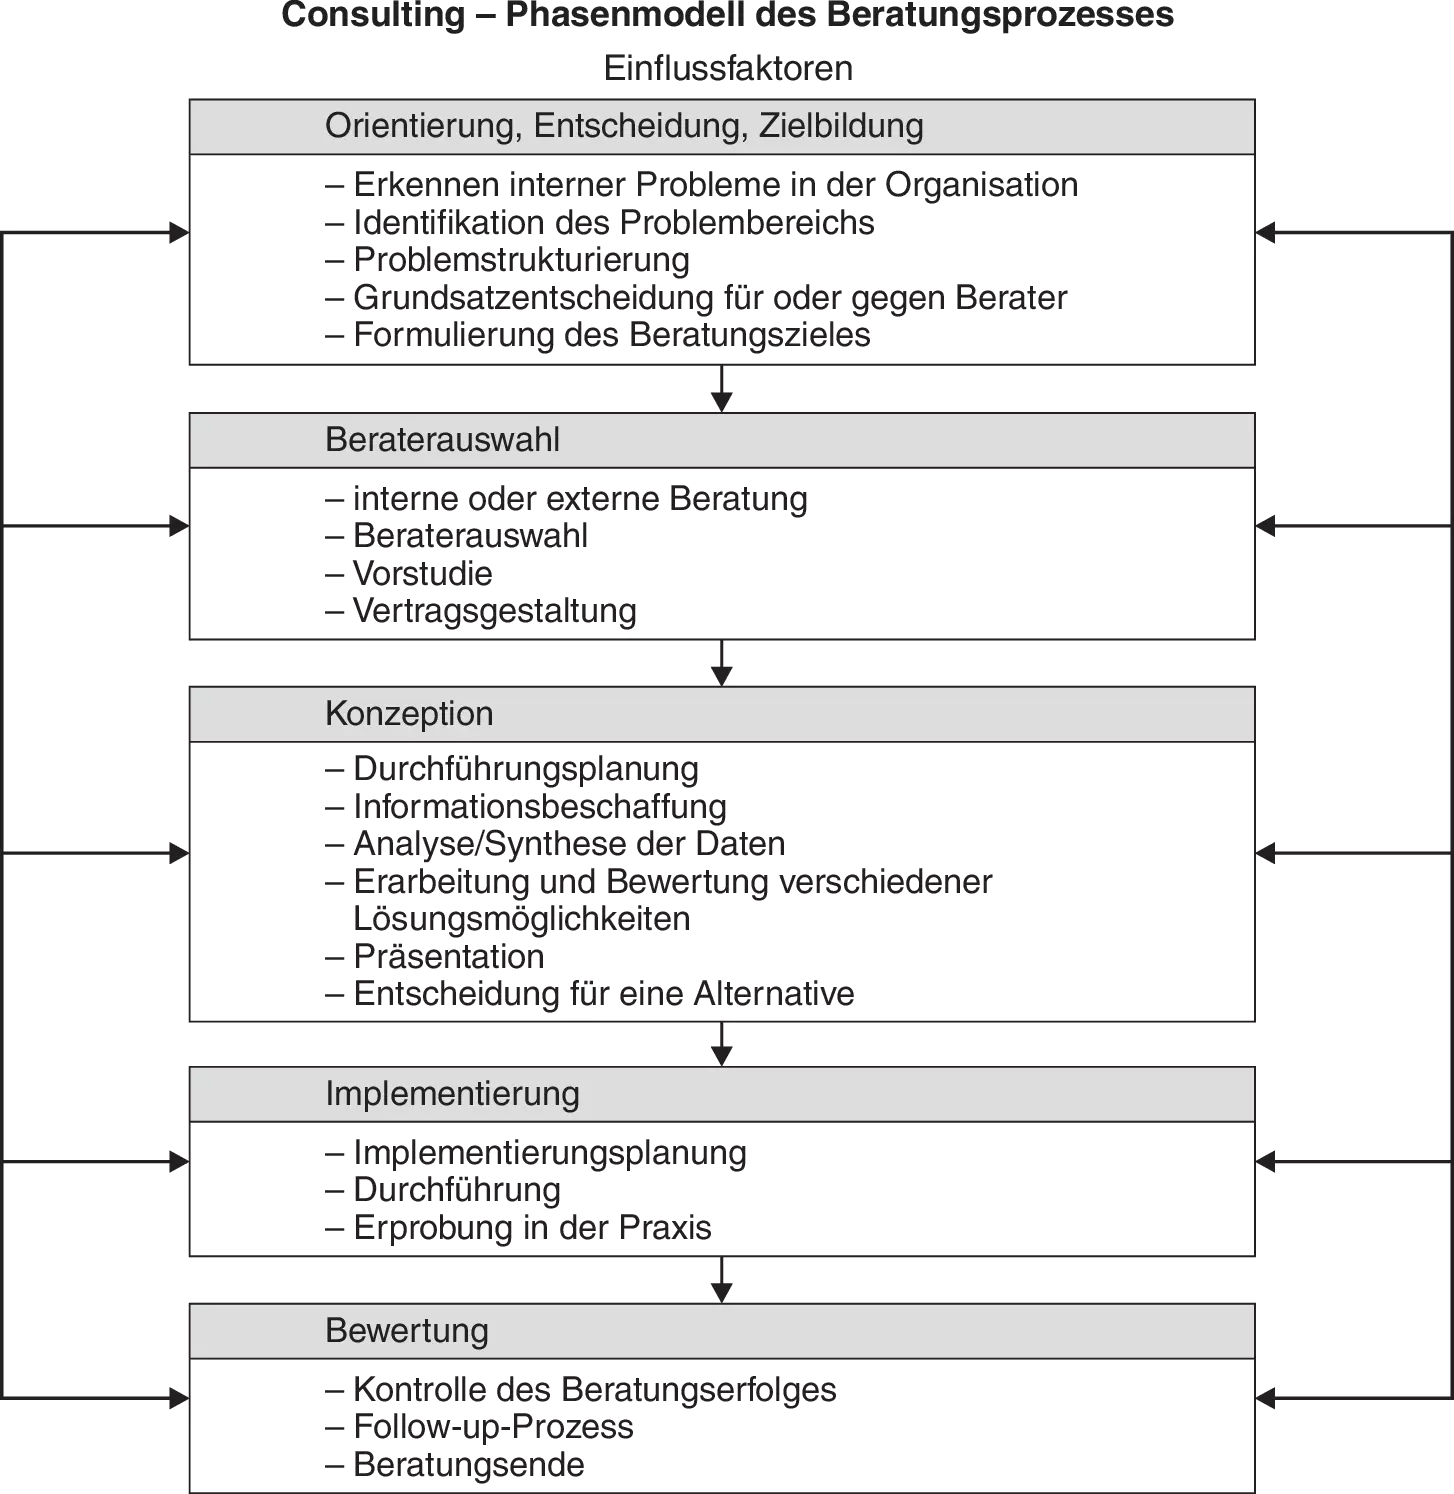
\includegraphics[scale=0.4]{./Bilder/Beratungsprozess.png}
    \caption[Phasenmodell eines Beratungsprozess]{Phasenmodell eines Beratungsprozess (Quelle: \cite[][]{gabler-beratung})}
\end{figure}
\\In der Praxis findet die Beratung in der Regel innerhalb von Projekten beim Kunden statt, die damit beginnen, dass der Kunde entweder auf das Beratungsunternehmen zukommt, oder eine Ausschreibung anfertigt, auf die sich das Beratungsunternehmen bewirbt. Danach erfolgt die Angebotserstellung durch das Beratungsunternehmen, in dem der Umfang des Projekts und die Leistungen der Berater festgehalten sind, sowie das Projektbudget. Die Abrechnung eines Projekts erfolgt entweder pauschal über einen Festpreis, oder über einen Stundensatz anhand der geleisteten Arbeitszeit. Sobald der Angebotszuschlag erhalten wurde, beginnt das Projekt mit der Konzeptionsphase, in der Informationen beschafft, Daten analysiert und verschiedene Lösungsmöglichkeiten in einem Fachkonzept erarbeitet werden. Sobald sich der Kunde für eine der Lösungen entschieden hat, beginnt mit der Implementierung die nächste Projektphase. In dieser findet die Durchführung der Lösung statt, sowie im Anschluss Tests und Fehlerbehebungen. Nach dem Abschluss der Implementierungsphase erfolgt die Abnahme, bzw. die Bewertung durch den Kunden, der auch eventuelle Nacharbeiten festsetzt oder nachfolgende Projekte in Aussicht stellt.\footcite[Vgl.][]{gabler-beratung}
\\Durch das nahende Supportende von SAP ERP (R/3) im Jahr 2027 (siehe Kapitel \ref{kap:R3}) stehen zurzeit viele Unternehmen unter Zugzwang auf die neuste Generation S/4HANA zu aktualisieren. Dadurch ergeben sich für die Beratungsbranche viele Möglichkeiten, Aufträge in Form von S/4HANA-Transformationsprojekten zu akquirieren. Auf der anderen Seite bietet der Druck auf die Unternehmen aber auch Chancen im selben Zug einschneidende Änderungen an den in SAP abgebildeten Geschäftsprozessen vorzunehmen, indem sich von Eigenentwicklungen und ineffizienten Prozessen getrennt wird und sie durch Prozesse des gängigen Industriestandards ersetzt.

\subsection{Vorgehensmodell S/4HANA Transformation}
\subsubsection{Aufbau}
Die adesso orange AG hat für die Durchführung von SAP S/4HANA Transformationen, mithilfe der im Unternehmen ansässigen Expertise, ein eigenes Vorgehensmodell entwickelt, dass auf verschiedenen Projektphasen und Bausteinen basiert, um eine Transformation von IT-Systemen und -Landschaften durchzuführen, vor allem aber auch um S/4HANA-Transformationen (siehe Kapitel \ref{kap:s4hanatrans}) zu vollziehen. Dieses Vorgehensmodell wird unter dem Produktnamen \glqq{}adesso active transformation\grqq{} vermarktet und kam bereits in einigen größeren S/4HANA-Transformation-Projekten zum Einsatz. Ziel dieses Vorgehensmodell ist, die Transformation strukturiert zu durchlaufen und dabei alle Aspekte von der Planung bis zur Umsetzung zu berücksichtigen. Wie bereits erwähnt, basiert das Modell auf verschiedenen Phasen, die wiederrum unterschiedliche Bausteine enthalten, die einzelne Leistungen abbilden, die z.B. in Form von Workshops (Arbeitsgruppen) oder Konzepten. Mithilfe dieser Bausteine, kann individuell, je nach Anforderungen der Kunden, ein Projekt effektiv durchgeplant werden. Des Weiteren werden während einer Transformation verschiedene \glqq{}Streams\grqq{} (Flüsse) betrachtet, die parallel zueinander laufen und sich durch das gesamte Projekt ziehen. Diese Streams bündeln die einzelnen Aktivitäten, z.B. technischer, organisatorischer, oder betriebswirtschaftlicher Natur sind. Das erklärte Hauptziel der \glqq{}adesso active transformation\grqq{} ist zum einen die Ermittlung eines optimalen Transformationspfads des betrachteten Systems, die Erstellung eines Umsetzungskonzeptes für die Transformation, sowie die letztendliche Umsetzung der Transformation in einer strukturierten Arbeitsweise.\footcite[Vgl.][]{aat-vorgehensmodell}

\subsubsection{Phasen}
Nachfolgend werden die einzelnen Projektphasen des Vorgehensmodell beschrieben, und ihre jeweiligen Bausteine zusammengefasst. In Abbildung \ref{fig:AAT} sind die einzelnen Phasen in einer Übersicht abgebildet.
\begin{figure}[!h]
    \centering
    \includegraphics[scale=0.65]{./Bilder/AAT-Überblick.png}
    \caption[Phasen des Vorgehensmodell]{Phasen der adesso active transformation (Quelle: \cite[][]{aat-phasen})}
    \label{fig:AAT}
\end{figure}
\\Das Vorgehensmodell beginnt mit der \underline{\glqq{}Enterprise Discover\grqq{}-Phase}, die das Ziel hat, das Kundenunternehmen für eine Transformation vorzubereiten und die strategischen Möglichkeiten der Vorgehensweise offen zulegen. In dieser Phase wird, wie der Name der Phase bereits andeutet, das Unternehmen, bzw. die Unternehmenslandschaft und Unternehmensarchitektur erkundet, um eine initiale Übersicht über das Unternehmen zu erhalten, mit allen Aspekten, die während einer Transformation berücksichtigt werden müssen. Des Weiteren finden diverse Beratungsgespräche zusammen mit den Kunden statt, in denen dem Kunden mögliche Wertschöpfungspotenziale und Gedankenanstöße für die Durchführung einer Transformation erörtert. Auch findet zu Beginn eine Evaluierung der Projektmethodik statt, in der entschieden wird, ob das Projekt, im Falle eines Angebotszuschlags durch den Kunden, klassisch nach Wasserfallmodell, agil oder als eine hybride Mischung der beiden Methodiken stattfinden soll. Zum Ende der Enterprise-Discover-Phase findet die Ermittlung des Projektumfangs statt, in der aufgelistet wird, wieviele zu transformierende Geschäftsprozesse es gibt, welche Prozesse neu abgebildet werden sollen, welche Werkzeuge im Projekt eingesetzt werden sollen und ob es übergreifende Themen gibt, die über das gesamte Projekt verteilt stattfinden müssen (z.B. Testmanagement). Dies ist zugleich auch das Ergebnisobjekt der ersten Phase und die Grundlage für die zweite Phase.\footcite[Vgl.][]{aat-enterprisediscover}\\
\vspace{1em}
\\Die zweite Phase in der adesso active transformation ist die \underline{\glqq{}Prepare\grqq{}-Phase}, die zum Ziel hat, die in der ersten Phase ermittelten Geschäftsprozesse ganzheitlich aufzunehmen und die Anforderungen aus der IT in Bezug auf die Transformation zu erfassen. Im Vorfeld findet jedoch zuerst eine UX-Journey (Vorstellung der Benutzeroberfläche) statt, in der ein neu aufgesetztes S/4HANA-System im Greenfield-Zustand dem Kunden präsentiert wird und dabei auf die Neuerungen eingegangen wird. Im Anschluss folgen weitere Präsentationen auf Modulebenen mit den jeweiligen Fachbereichen des Unternehmen, in denen weitere Anforderungen an die Transformation ermittelt werden. Die Ergebnisse dieser Vorstellungen wird im Anschluss dokumentiert und zusammengefasst und dienen der Definition des Tranformationspfads, also welcher Ansatz zur S/4HANA-Transformation verfolgt werden soll. Ebenfalls werden in der Prepare-Phase die momentanen Reporting- und Planungsprozesse aufgenommen und die neuen Business Intelligence Funktionen von SAP S/4HANA präsentiert. Zum Ende dieser Phase werden die einzelnen Ergebnisobjekte zu einem ersten Konzept konsolidiert, das als Basis der dritten Phase dient. Am Ende der Prepare-Phase steht ein \glqq{}Quality Gate\grqq{}, also eine Abnahme durch den Kunden, in der Kunde überprüft, ob die an das Projekt gestellten Anforderungen erfüllt werden.\footcite[Vgl.][]{aat-prepare}\\
\vspace{1em}
\\Die dritte Phase in der adesso active transformation ist die \underline{\glqq{}Explore\grqq{}-Phase}, die zum Ziel hat, die Ergebnisse der zweiten Phase in ein Feinkonzept zu überführen. Ebenfalls erfolgt in dieser Phase die Vorbereitung der technischen Systeme auf die Umsetzung in der nächsten Phase. Diese Vorbereitung besteht zu einem aus der Aufsetzung von Entwicklungs-, Test- und Produktivsystemen, aber auch aus der Bereitstellung der Systemzugänge für die Projektmitarbeiter in den neuen, sowie in den alten Systemen. Ein weiterer Punkt in der Explore-Phase ist das Thema Authentifizierung und Sicherheit, indem es zum einen um die Sicherheit des System, also um das Erstellen eines Rollen- und Berechtigungskonzept geht, in dem entweder die Übernahme von bestehenden Strukturen beschlossen wird, oder ein kompletter Neuaufbau der Rollen und Berechtigungen beschrieben ist. Zum anderen geht es aber auch um die Datensicherheit, in dem regelmäßige Datensicherungen durchgeführt werden und die Anforderungen der europäischen Datenschutz Grundverordnung (EU-DSGVO) zum Speichern von personenbezogenen Daten erfüllt werden müssen. Das Ergebnisobjekt der Prepare-Phase ist das Feinkonzept, was die Basis für die Umsetzung in der nächsten Phase darstellt.\footcite[Vgl.][]{aat-explore}\\
\vspace{1em}
\\In der vierten Phase, der \underline{\glqq{}Realize\grqq{}-Phase}, geht es schließlich um die Umsetzung des Feinkonzepts. Dies geschieht, indem das neue System konfiguriert und an die Bedürfnisse des Kunden angepasst wird. Dazu werden, je nach Konzept, die Geschäftsprozesse des Unternehmen neu im System abgebildet oder aus dem Altsystem übernommen. Ebenfalls werden die nach wie vor benötigten Eigenentwicklungen entweder übernommen oder im S/4HANA neu aufgebaut. Da je nach Projekt auch historische Daten aus dem Altsystem übernommen werden, müssen auch die in das neue System migriert werden. Aufgrund der Änderungen in der Datenstruktur in S/4HANA müssen hierzu Umschlüsselungen der Datenbanktabellen stattfinden, damit die Daten übernommen werden können. Ein weiteres wichtiges Thema ist das anschließende Testen des Systems und der Prozesse. Dies muss strukturiert erfolgen, damit alle Geschäftsprozesse, in allen Variationen, vollständig getestet werden, um Fehler zu erkennen und diese zu beheben. Zum Ende der Realize-Phase erfolgt die Abnahme durch den Kunden, in der überprüft wird, ob alle Prozesse und Systeme wie gewünscht funktionieren, alle Anforderungen erfüllt wurden und ob das S/4HANA-System in den produktiven Betrieb gehen kann.\footcite[Vgl.][]{aat-realize}\\
\vspace{1em}
\\Der \underline{\glqq{}Go-Live\grqq{}} und die anschließenden Nacharbeiten stellen die fünfte Projektphase in der adesso active transformation dar. Hierbei erfolgt nach der erfolgreichen Abnahme des Systems durch den Kunden, der Go-Live, also die Produktivsetzung des Systems. Da, aufgrund der intensiven Nutzung nach Go-Live, häufig auch dann noch Fehler auftreten, werden diese durch das Projektteam nach Go-Live behoben. Auch kann es vorkommen, dass in diesem Zeitraum noch nachgelagerte Aktivitäten stattfinden, die von Vorhinein niedrig priorisiert wurden. Ebenfalls werden in diesem Zeitraum häufig die Dokumentationen und die Anwenderhandbücher noch finalisiert und dem Kunden übergeben. Nach der Go-Live-Phase kann durch den Kunden noch ein individueller Wartungsvertrag geschlossen werden, in dem definiert ist, dass auch nach Ende des Projekts Fehlerbehebungen stattfinden.\footcite[Vgl.][]{aat-golive}


\subsubsection{Werkzeuge}
Das adesso active Transformation Vorgehensmodell sieht neben den verschiedenen Projektphasen auch phasenübergreifende Werkzeug vor, die zum Einsatz kommen und die Projektmitarbeiter unterstützen soll. \\Dies ist zum einen die Webanwendung \underline{\glqq{}Jira\grqq{}} vom Softwarehersteller Atlassian, die sich für die systematische Projektsteuerung und das Nachverfolgen von Aufgaben eignet, aber auch Funktionen für das Melden von Fehlern (bug reporting) vorsieht. In Jira lassen sich verschiedene Teilprojekte in Form von Komponenten aufbauen und Meilensteine in Form von Releases abbilden. Für das Vorgehensmodell ist eine Jira-Vorlage vorgesehen, mit dem ein Projekt in Jira angelegt werden kann, indem bereits die Grundkonfiguration vorgenommen wurde.\\
Ebenfalls ist in der adesso active transformation eine Excel-Spreadsheet-Vorlage zur Durchführung des Projektcontrollings vorgesehen. Dieses Spreadsheet dient zur Unterstützung der Projektleitung, indem diese das Projektbudget verwalten und den Einsatz der Projektmitarbeiter planen kann. Sobald das Spreadsheet an das entsprechende Projekt angepasst und konfiguriert ist, können die vorgesehenen Projekttage der Projektmitarbeiter erfasst und über den gesamten Projektzeitraum vorausgeplant werden.  
Das Tool ermöglicht zudem den Import von erfassten Arbeitszeiten über eine Schnittstelle zu dem von adesso orange eingesetzten Zeiterfassungstool \glqq{}ZEP\grqq{}. Somit kann die Projektleitung zu jedem Zeitpunkt einen Soll-Ist-Vergleich vornehmen und ggf. das Budget umverteilen oder zusätzliche Projekttage beantragen.

\subsubsection{Business Transformation Tracker}
Ein weiteres wichtiges Tool im Vorgehensmodell ist der \underline{\glqq{}Business Transformation Tracker\grqq{}} (BTT) der zum momentanen Zeitpunkt durch ein Excel-Spreadsheet implementiert ist. In diesem werden zu Beginn des Projektes, in der Prepare-Phase, die Geschäftsprozesse, die es zu transformieren gilt, ganzheitlich erfasst. Dazu werden die Prozesse in Subprozesse und Prozessschritte aufgespalten und Schritt für Schritt in dem Business Transformation Tracker eingetragen. Im BTT sind je Projektphase verschiedene Kriterien hinterlegt, durch die die Vollständigkeit der Transformation je Prozessschritt ermittelt wird. Diese Kriterien können entweder Eigenschaften oder Aufgaben sein, deren Erfüllung im BTT dokumentiert wird. In der Regel gibt es pro Teilprojekt im Transformationsprojekt einen Business Transformation Tracker in Form eines Excel-Spreadsheets.\\
Da diese Umsetzung schnell unübersichtlich wird und der Funktionsumfang auch nur begrenzt ist, besteht bei adesso orange der Wunsch, die momentan implementierte Excel-Lösung in ein eigenes System zu überführen. Die Konzeption dieser Überführung in ein eigenständiges Systems wird nun in den folgenden Kapiteln behandelt.